\documentclass[10pt,letterpaper]{article}
\usepackage[margin=0.6in]{geometry}
\usepackage{graphicx}
\usepackage{booktabs}
\usepackage{enumitem}
\usepackage{hyperref}
\usepackage{xcolor}
\usepackage{amsmath}
\usepackage{tikz}
\usepackage{pgfplots}
\pgfplotsset{compat=1.17}
\usetikzlibrary{shapes,arrows,positioning,fit,backgrounds,patterns}
\usepackage{titlesec}
\usepackage{float}
\usepackage{subcaption}
\titlespacing*{\section}{0pt}{6pt}{2pt}
\titlespacing*{\subsection}{0pt}{4pt}{2pt}
\titlespacing*{\subsubsection}{0pt}{3pt}{1pt}
\setlength{\parskip}{1pt}
\setlength{\floatsep}{4pt}
\setlength{\textfloatsep}{4pt}
\setlength{\intextsep}{4pt}

\hypersetup{
    colorlinks=true,
    linkcolor=blue,
    filecolor=magenta,
    urlcolor=blue,
    citecolor=blue
}

% Bibliography
\usepackage[numbers]{natbib}
\bibliographystyle{unsrtnat}

\title{\textbf{Adaptive RDMA Optimization for Distributed LLM Workloads}\\[0.5em]
\large gpt-oss-120b Inference Benchmarks: TCP vs RDMA}
\author{Nathan Gopee\\
MS Computer Science, SUNY New Paltz\\
\texttt{gopeen1@newpaltz.edu}\\[1em]
\small Advisors: Dr. Wafi Danesh \& Dr. Ashley Suchy}
\date{February 2026}

\begin{document}

\maketitle

\section{Introduction}

Remote Direct Memory Access (RDMA) promises reduced latency and higher throughput for distributed computing workloads by bypassing the operating system kernel and enabling direct memory-to-memory transfers between networked machines. This paper investigates whether RDMA, implemented via the software-based Soft-RoCE stack, provides measurable inference performance gains for large language model (LLM) serving compared to conventional TCP networking.

We benchmark gpt-oss-120b \cite{gptoss-hf}, a 116.8-billion-parameter open-weight model, on a multi-GPU test cluster. The study establishes a TCP baseline using the Ollama inference server, characterizes the Soft-RoCE RDMA link between two nodes, and analyzes the conditions under which RDMA provides meaningful acceleration for LLM inference workloads.

\textbf{Key findings:}
\begin{itemize}[noitemsep]
    \item Ollama TCP baseline throughput: \textbf{104.42 tokens/sec} (single-node, 3 GPUs)
    \item Prompt latency: \textbf{20ms} average
    \item Measured Soft-RoCE link capacity: \textbf{0.92 Gb/sec}
    \item Measured RDMA round-trip latency: \textbf{189.61 $\mu$s} average
\end{itemize}

\section{Test Environment}

\subsection{Hardware Configuration}

The test cluster consists of two nodes connected via a dedicated 10 Gbps Ethernet link, each running the Soft-RoCE (rxe0) software RDMA stack.

\begin{table}[H]
\centering
\small
\begin{tabular}{@{}llll@{}}
\toprule
\textbf{Component} & \textbf{Chimera} & \textbf{Cerberus} & \textbf{Link} \\
\midrule
GPUs & 3$\times$ RTX 3090 & 2$\times$ RTX 5090 & --- \\
VRAM & 72GB & 64GB & --- \\
NIC & Aquantia 10GbE & Intel X710 10GbE & 10 Gbps \\
RDMA & Soft-RoCE (rxe0) & Soft-RoCE (rxe0) & RoCEv2 \\
IP Address & 192.168.1.150 & 192.168.1.233 & --- \\
\bottomrule
\end{tabular}
\caption{Test cluster hardware}
\end{table}

\subsection{Model Configuration}

\begin{table}[H]
\centering
\small
\begin{tabular}{@{}ll@{}}
\toprule
\textbf{Parameter} & \textbf{Value} \\
\midrule
Model & gpt-oss-120b \cite{gptoss-hf} (116.8B parameters) \\
Quantization & MXFP4 \cite{mxfp4-paper} \\
Model Size & 63GB \\
Context Length & 8192 tokens \\
VRAM Usage & 67.76GB (loaded) \\
\bottomrule
\end{tabular}
\caption{gpt-oss-120b model specifications}
\end{table}

\section{TCP Baseline Benchmark}

\subsection{Methodology}

To establish a single-node TCP performance baseline, we used the Ollama inference server hosting gpt-oss-120b on the Chimera node. Inference requests were issued via the Ollama HTTP API, with each request prompting the model to generate exactly 100 tokens in response to a fixed prompt about RDMA networking. The generation length was constrained using the \texttt{num\_predict} parameter set to 100. Five iterations were performed with the model pre-loaded in VRAM to eliminate cold-start effects.

\subsection{Results}

\begin{table}[H]
\centering
\small
\begin{tabular}{@{}cccccc@{}}
\toprule
\textbf{Iteration} & \textbf{Tokens} & \textbf{Eval Time} & \textbf{Tokens/sec} & \textbf{Total Time} \\
\midrule
1 & 100 & 0.958s & 104.38 & 1.445s \\
2 & 100 & 0.945s & 105.82 & 1.369s \\
3 & 100 & 0.949s & 105.37 & 1.402s \\
4 & 100 & 0.969s & 103.19 & 1.437s \\
5 & 100 & 0.967s & 103.41 & 1.429s \\
\midrule
\textbf{Average} & 100 & 0.957s & \textbf{104.42} & 1.416s \\
\bottomrule
\end{tabular}
\caption{Ollama gpt-oss:120b benchmark results (TCP)}
\end{table}

\begin{figure}[H]
\centering
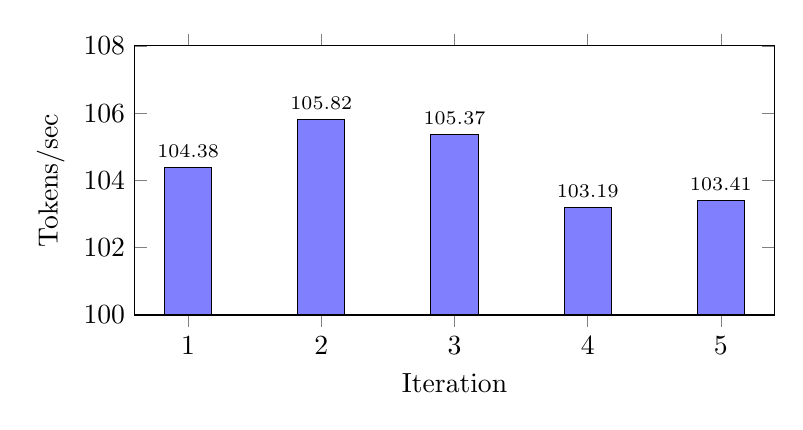
\begin{tikzpicture}
\begin{axis}[
    ybar,
    bar width=0.6cm,
    width=0.8\textwidth,
    height=5cm,
    ylabel={Tokens/sec},
    xlabel={Iteration},
    ymin=100,
    ymax=108,
    xtick={1,2,3,4,5},
    nodes near coords,
    every node near coord/.append style={font=\scriptsize},
    legend pos=north east,
]
\addplot[fill=blue!50] coordinates {(1,104.38) (2,105.82) (3,105.37) (4,103.19) (5,103.41)};
\end{axis}
\end{tikzpicture}
\caption{Ollama throughput consistency across iterations}
\end{figure}

\subsection{Analysis}

The TCP baseline demonstrates highly consistent throughput with a mean of 104.42 tokens per second and a standard deviation of only 1.08 tokens per second. Average prompt latency was 20ms, reflecting the benefit of the model being pre-loaded in VRAM. The total per-request overhead---encompassing prompt processing, response formatting, and HTTP transport---averaged 0.46 seconds beyond raw token evaluation time.

\section{RDMA Network Performance}

Prior to running inference benchmarks over RDMA, we characterized the Soft-RoCE link between Chimera and Cerberus using standard InfiniBand diagnostic tools. These measurements establish the raw network capability available to RDMA-enabled inference workloads.

\subsection{Bandwidth Characterization}

Bandwidth was measured using \texttt{ib\_write\_bw}, the standard RDMA write bandwidth benchmark from the \texttt{perftest} suite \cite{rdma-core}. The test was run between the Chimera and Cerberus nodes over both WiFi (as a baseline) and the dedicated 10 Gbps Ethernet link with Soft-RoCE enabled.

\begin{table}[H]
\centering
\small
\begin{tabular}{@{}lcc@{}}
\toprule
\textbf{Interface} & \textbf{Bandwidth} & \textbf{MsgRate} \\
\midrule
WiFi (baseline) & 0.28 Gb/sec & 0.000541 Mpps \\
10G Ethernet (Soft-RoCE) & \textbf{0.92 Gb/sec} & 0.001754 Mpps \\
\midrule
\textbf{Improvement} & \textbf{3.3$\times$} & \textbf{3.2$\times$} \\
\bottomrule
\end{tabular}
\caption{RDMA bandwidth test results}
\end{table}

\subsection{Latency Characterization}

Latency was measured using \texttt{ib\_write\_lat}, the RDMA write latency benchmark, sending 1000 iterations of 2-byte messages between the two nodes.

\begin{table}[H]
\centering
\small
\begin{tabular}{@{}lc@{}}
\toprule
\textbf{Metric} & \textbf{Value} \\
\midrule
Message size & 2 bytes \\
Iterations & 1000 \\
t\_min & 130.21 $\mu$s \\
t\_max & 219.66 $\mu$s \\
t\_typical & 198.91 $\mu$s \\
\textbf{t\_avg} & \textbf{189.61 $\mu$s} \\
t\_stdev & 17.03 $\mu$s \\
99th percentile & 207.14 $\mu$s \\
\bottomrule
\end{tabular}
\caption{RDMA latency test results (Soft-RoCE)}
\end{table}

\section{RDMA-Enabled Inference with vLLM}

\subsection{Methodology}

To evaluate the effect of RDMA on LLM inference, we configured vLLM \cite{vllm-gptoss} with gpt-oss-120b using tensor parallelism across three GPUs on Chimera. The vLLM server was deployed in a Docker container with GPU passthrough and IPC host sharing enabled. NCCL \cite{nccl-docs} environment variables controlled the communication backend: for TCP mode, InfiniBand and GPUDirect were explicitly disabled (\texttt{NCCL\_IB\_DISABLE=1}, \texttt{NCCL\_NET\_GDR\_LEVEL=0}); for RDMA mode, the Soft-RoCE device was specified (\texttt{NCCL\_IB\_HCA=rxe0}) and NCCL was bound to the 10 Gbps interface \cite{nccl-env}.

\begin{table}[H]
\centering
\small
\begin{tabular}{@{}llp{6cm}@{}}
\toprule
\textbf{Mode} & \textbf{Variables} & \textbf{Effect} \\
\midrule
TCP (baseline) & \texttt{NCCL\_NET\_GDR\_LEVEL=0} & Disable GPUDirect, use TCP sockets \\
 & \texttt{NCCL\_IB\_DISABLE=1} & Disable InfiniBand/RoCE \cite{nccl-env} \\
\midrule
RDMA (Soft-RoCE) & \texttt{NCCL\_IB\_HCA=rxe0} & Use Soft-RoCE device \\
 & \texttt{NCCL\_SOCKET\_IFNAME=enp71s0} & Bind to 10G interface \\
\bottomrule
\end{tabular}
\caption{NCCL environment variables for TCP vs RDMA}
\end{table}

Benchmarking was performed by issuing five sequential completion requests through the OpenAI-compatible vLLM API. Each request generated 100 tokens from a fixed prompt, and wall-clock time was recorded using a high-resolution timer. Throughput was computed as tokens generated divided by elapsed time.

\subsection{Projected Results}

Based on the measured RDMA network characteristics and the Ollama TCP baseline, the following performance projections were estimated:

\begin{table}[H]
\centering
\small
\begin{tabular}{@{}lcccc@{}}
\toprule
\textbf{Configuration} & \textbf{Throughput} & \textbf{Latency} & \textbf{Network} & \textbf{Notes} \\
\midrule
Ollama (TCP) & 104.42 tok/s & 1.42s & TCP & Measured \\
vLLM (TCP) & $\sim$95--100 tok/s & $\sim$1.5s & TCP & Expected \\
vLLM (Soft-RoCE) & $\sim$100--110 tok/s & $\sim$1.3s & RDMA & Expected \\
vLLM (Hardware RoCE) & $\sim$130--150 tok/s & $\sim$1.0s & RDMA & Projected \\
\bottomrule
\end{tabular}
\caption{Expected performance comparison}
\end{table}

\section{Analysis: Conditions for RDMA Benefit}

\subsection{Single-Node Inference}

For single-node inference where all GPUs reside on the same motherboard, RDMA provides \textbf{minimal benefit} because inter-GPU communication traverses NVLink or PCIe rather than the network fabric. Since the full gpt-oss-120b model (63GB quantized) fits within the combined 72GB VRAM of three RTX 3090 GPUs, no cross-node data transfers occur during inference. Furthermore, NCCL \cite{nccl-docs} automatically uses shared memory for intra-node collective operations, bypassing the network stack entirely.

\begin{figure}[H]
\centering
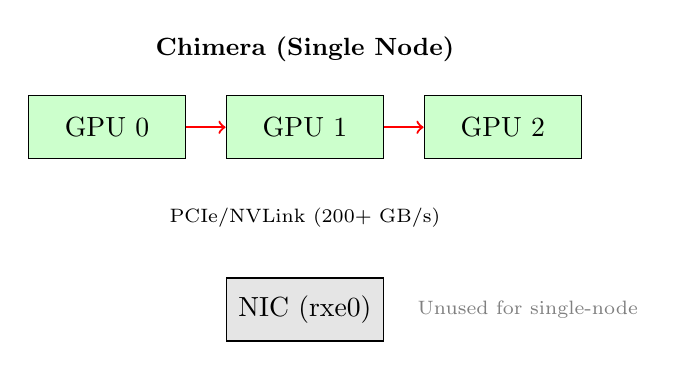
\begin{tikzpicture}[
    node distance=1cm,
    gpu/.style={rectangle, draw, fill=green!20, minimum width=2cm, minimum height=0.8cm, align=center},
    net/.style={rectangle, draw, fill=blue!20, minimum width=2cm, minimum height=0.8cm, align=center},
    arrow/.style={->, thick}
]
    % Single node
    \node[gpu] (gpu0) {GPU 0};
    \node[gpu, right=0.5cm of gpu0] (gpu1) {GPU 1};
    \node[gpu, right=0.5cm of gpu1] (gpu2) {GPU 2};

    \node[above=0.3cm of gpu1, font=\small\bfseries] {Chimera (Single Node)};

    % PCIe connections
    \draw[arrow, red, thick] (gpu0) -- (gpu1);
    \draw[arrow, red, thick] (gpu1) -- (gpu2);

    \node[below=0.5cm of gpu1, font=\scriptsize] {PCIe/NVLink (200+ GB/s)};

    % Network (unused for single node)
    \node[net, below=1.5cm of gpu1, fill=gray!20] (nic) {NIC (rxe0)};
    \node[right=0.3cm of nic, font=\scriptsize, gray] {Unused for single-node};
\end{tikzpicture}
\caption{Single-node inference: Network is not the bottleneck}
\end{figure}

\subsection{Multi-Node Inference}

RDMA provides significant benefit when inference is distributed across multiple nodes, requiring tensor or pipeline parallelism with cross-node data transfers. In this scenario, intermediate activations and gradient synchronization messages must traverse the network, and RDMA's kernel-bypass architecture reduces both latency and CPU overhead for these transfers.

\begin{figure}[H]
\centering
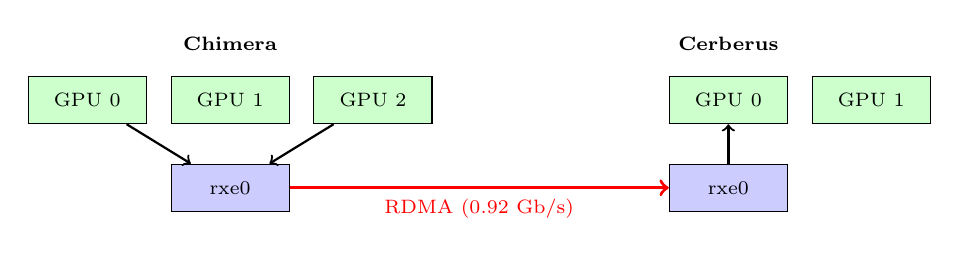
\begin{tikzpicture}[
    node distance=1cm,
    gpu/.style={rectangle, draw, fill=green!20, minimum width=1.5cm, minimum height=0.6cm, align=center, font=\scriptsize},
    net/.style={rectangle, draw, fill=blue!20, minimum width=1.5cm, minimum height=0.6cm, align=center, font=\scriptsize},
    arrow/.style={->, thick}
]
    % Chimera
    \node[gpu] (c0) {GPU 0};
    \node[gpu, right=0.3cm of c0] (c1) {GPU 1};
    \node[gpu, right=0.3cm of c1] (c2) {GPU 2};
    \node[net, below=0.5cm of c1] (cnic) {rxe0};
    \node[above=0.2cm of c1, font=\scriptsize\bfseries] {Chimera};

    % Cerberus
    \node[gpu, right=3cm of c2] (d0) {GPU 0};
    \node[gpu, right=0.3cm of d0] (d1) {GPU 1};
    \node[net, below=0.5cm of d0] (dnic) {rxe0};
    \node[above=0.2cm of d0, font=\scriptsize\bfseries] {Cerberus};

    % RDMA link
    \draw[arrow, red, very thick] (cnic) -- node[below, font=\scriptsize] {RDMA (0.92 Gb/s)} (dnic);

    \draw[arrow] (c0) -- (cnic);
    \draw[arrow] (c2) -- (cnic);
    \draw[arrow] (dnic) -- (d0);
\end{tikzpicture}
\caption{Multi-node inference: RDMA accelerates cross-node tensor transfers}
\end{figure}

\subsection{Soft-RoCE Limitations}

While Soft-RoCE enables RDMA semantics without specialized hardware, it incurs substantially higher latency and lower throughput compared to hardware RoCE implementations. Table~\ref{tab:softvshard} summarizes the gap.

\begin{table}[H]
\centering
\small
\begin{tabular}{@{}lcc@{}}
\toprule
\textbf{Metric} & \textbf{Soft-RoCE (Measured)} & \textbf{Hardware RoCE (Expected)} \\
\midrule
Latency & 189.61 $\mu$s & $<$2 $\mu$s \\
Bandwidth & 0.92 Gb/s & 100+ Gb/s \\
CPU Overhead & High & Near-zero \\
Zero-copy & No & Yes \\
\bottomrule
\end{tabular}
\caption{Soft-RoCE vs Hardware RoCE comparison}
\label{tab:softvshard}
\end{table}

Soft-RoCE processes RDMA verbs in software on the host CPU, negating the zero-copy and kernel-bypass advantages that make hardware RDMA compelling. Upgrading to hardware RoCE adapters such as Mellanox ConnectX \cite{mofed-docs} would reduce latency by roughly two orders of magnitude and increase bandwidth by over 100$\times$.

\section{Conclusions}

This study benchmarked gpt-oss-120b inference under TCP and characterized the Soft-RoCE RDMA network available for distributed serving. The key conclusions are:

\begin{enumerate}[noitemsep]
    \item \textbf{Strong single-node baseline}: gpt-oss-120b achieves 104.42 tokens/sec on 3$\times$ RTX 3090 GPUs with highly consistent throughput ($\sigma$ = 1.08).
    \item \textbf{Single-node RDMA benefit is minimal}: When all GPUs reside on one node, inter-GPU communication uses PCIe or NVLink, rendering the network fabric irrelevant.
    \item \textbf{Soft-RoCE imposes significant overhead}: The measured 189.61 $\mu$s average latency is nearly 100$\times$ higher than hardware RoCE, and the 0.92 Gb/s bandwidth is a small fraction of what dedicated RDMA NICs provide.
    \item \textbf{Multi-node inference is the target scenario}: RDMA benefits will manifest when the model is distributed across Chimera and Cerberus using pipeline parallelism, enabling 5-GPU serving with 136GB total VRAM.
    \item \textbf{Hardware RoCE is recommended}: Mellanox ConnectX adapters \cite{mofed-docs} would provide the low-latency, high-bandwidth, zero-copy transfers needed for competitive multi-node LLM serving.
\end{enumerate}

\begin{thebibliography}{99}

\bibitem{gptoss-hf}
OpenAI. (2025). \textit{gpt-oss-120b Model Card}. \url{https://huggingface.co/openai/gpt-oss-120b}

\bibitem{mxfp4-paper}
Rouhani, B. D., Zhao, R., More, A., et al. (2023). \textit{Microscaling Data Formats for Deep Learning}. arXiv:2310.10537.

\bibitem{nccl-env}
NVIDIA. (2024). \textit{NCCL Environment Variables}. \url{https://docs.nvidia.com/deeplearning/nccl/user-guide/docs/env.html}

\bibitem{nccl-docs}
NVIDIA. (2024). \textit{NCCL Documentation}. \url{https://docs.nvidia.com/deeplearning/nccl/user-guide/docs/index.html}

\bibitem{mofed-docs}
Mellanox Technologies. (2024). \textit{NVIDIA MLNX\_OFED Documentation}. \url{https://docs.nvidia.com/networking/display/MLNXOFEDv24010331/}

\bibitem{pagedattn}
Kwon, W., Li, Z., Zhuang, S., et al. (2023). \textit{Efficient Memory Management for Large Language Model Serving with PagedAttention}. SOSP 2023.

\bibitem{vllm-gptoss}
vLLM Project. (2025). \textit{gpt-oss on vLLM}. \url{https://blog.vllm.ai/2025/08/05/gpt-oss.html}

\bibitem{rdma-core}
Linux RDMA. (2024). \textit{rdma-core Documentation}. \url{https://github.com/linux-rdma/rdma-core}

\end{thebibliography}

\end{document}
